\documentclass{standalone}
\usepackage{tikz}
\usetikzlibrary{patterns, positioning}
\usepackage[sfdefault]{ClearSans} %% option 'sfdefault' activates Clear Sans as the default text font
\usepackage[T1]{fontenc}

\begin{document}
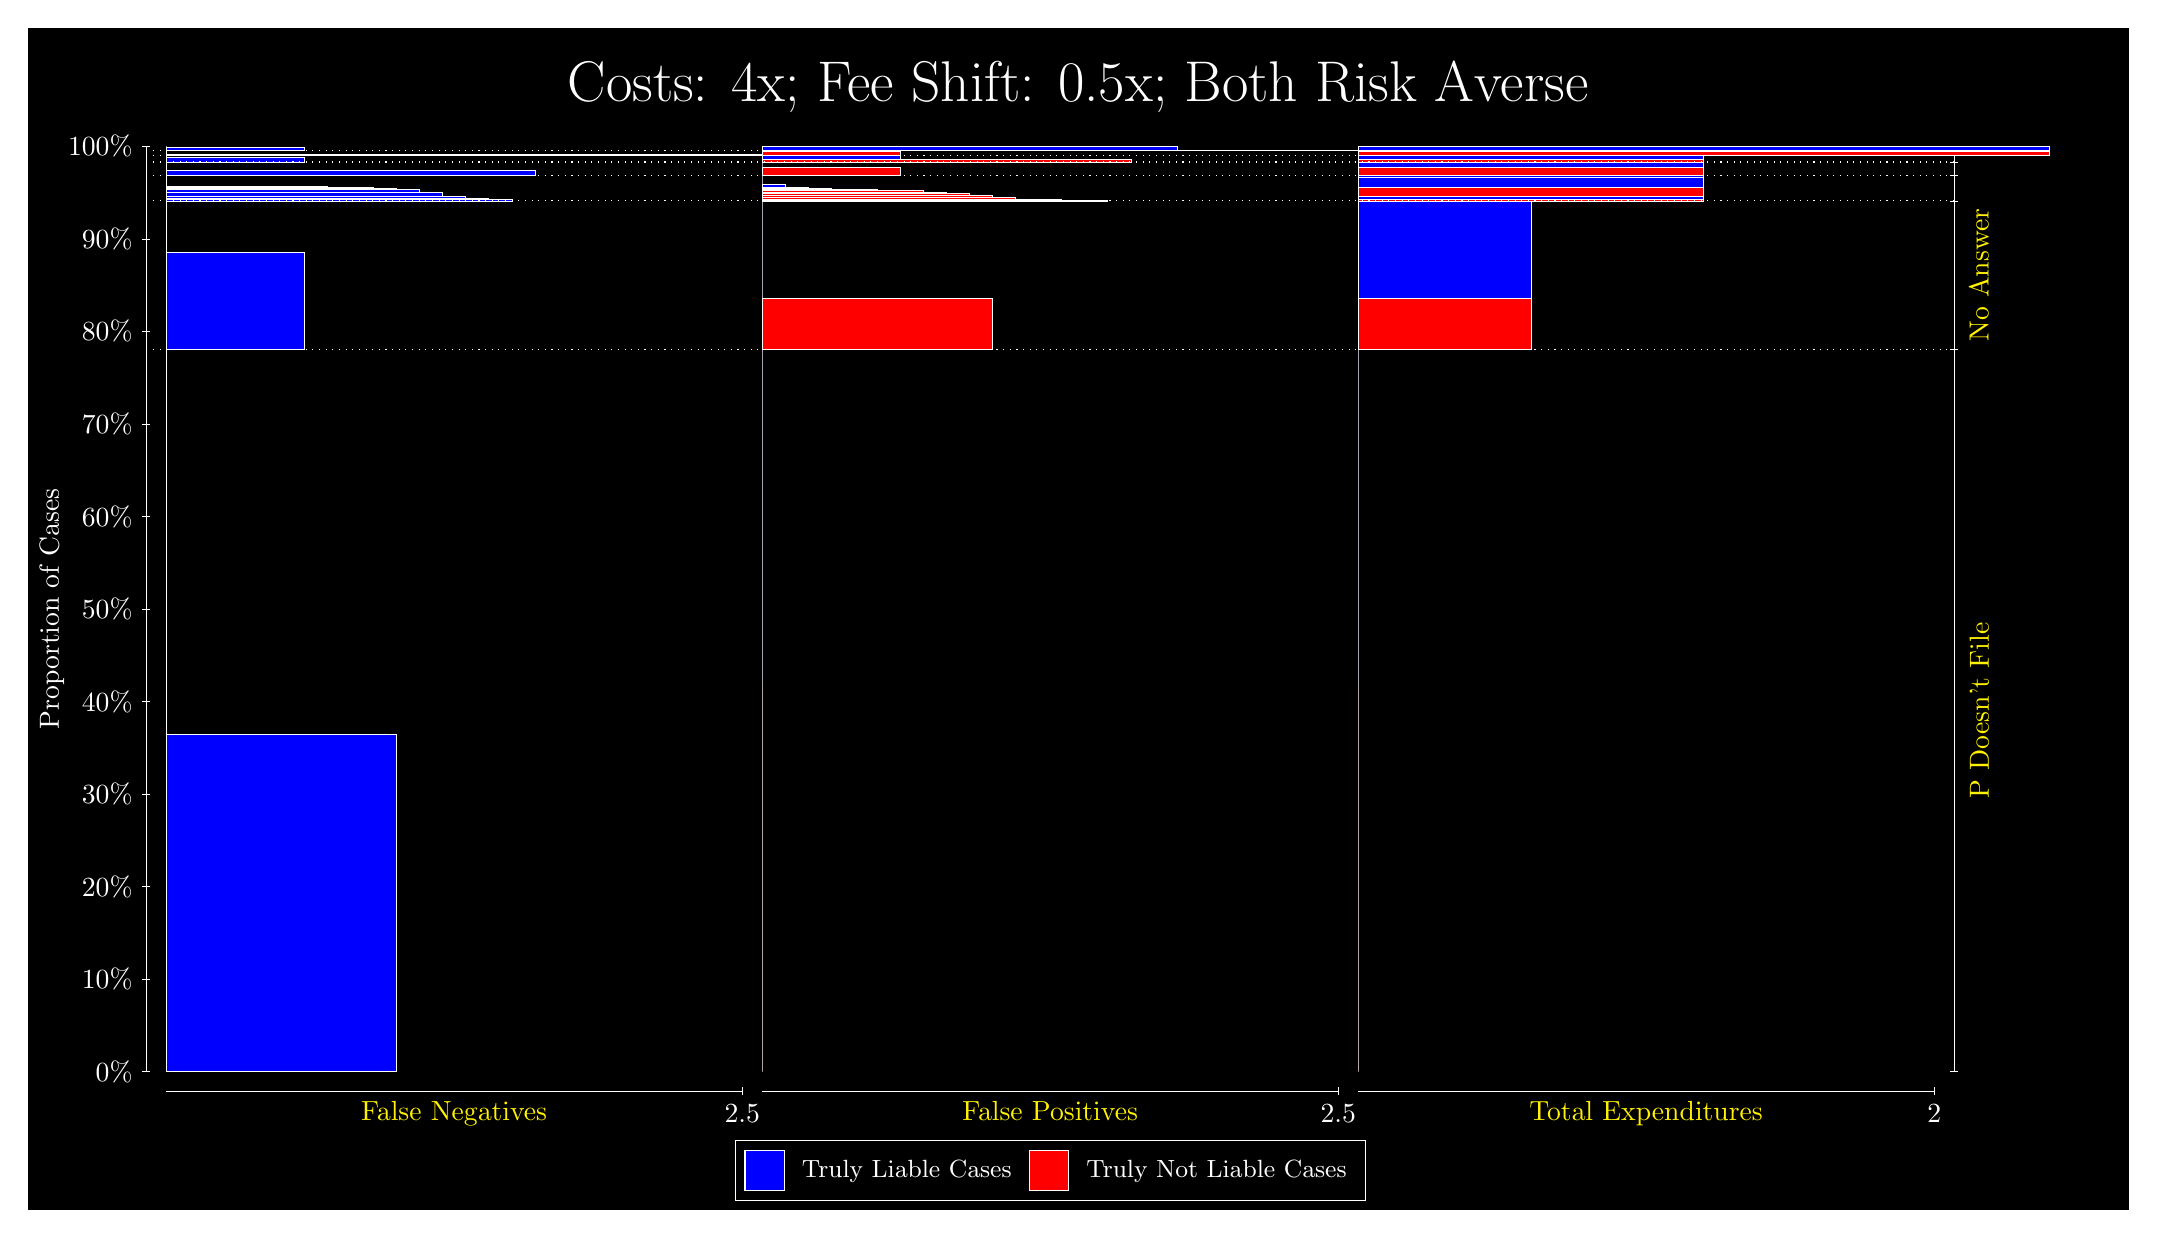
\begin{tikzpicture}
\draw[fill=black] (0,0) rectangle (26.667,15);
\draw[text=white] (0,13.5) rectangle (26.667,15) node[midway] {\huge Costs: 4x; Fee Shift: 0.5x; Both Risk Averse};
\draw[white, very thin] (1.5,1.75) -- (1.5,13.5);
\node[rotate=90, text=white, anchor=center] at (0.3, 7.625) {Proportion of Cases};
\draw[white, very thin] (1.45,1.75) -- (1.55,1.75);
\node[text=white, anchor=east] at (1.45, 1.75) {0\%};
\draw[white, very thin] (1.45,2.925) -- (1.55,2.925);
\node[text=white, anchor=east] at (1.45, 2.925) {10\%};
\draw[white, very thin] (1.45,4.1) -- (1.55,4.1);
\node[text=white, anchor=east] at (1.45, 4.1) {20\%};
\draw[white, very thin] (1.45,5.275) -- (1.55,5.275);
\node[text=white, anchor=east] at (1.45, 5.275) {30\%};
\draw[white, very thin] (1.45,6.45) -- (1.55,6.45);
\node[text=white, anchor=east] at (1.45, 6.45) {40\%};
\draw[white, very thin] (1.45,7.625) -- (1.55,7.625);
\node[text=white, anchor=east] at (1.45, 7.625) {50\%};
\draw[white, very thin] (1.45,8.8) -- (1.55,8.8);
\node[text=white, anchor=east] at (1.45, 8.8) {60\%};
\draw[white, very thin] (1.45,9.975) -- (1.55,9.975);
\node[text=white, anchor=east] at (1.45, 9.975) {70\%};
\draw[white, very thin] (1.45,11.15) -- (1.55,11.15);
\node[text=white, anchor=east] at (1.45, 11.15) {80\%};
\draw[white, very thin] (1.45,12.325) -- (1.55,12.325);
\node[text=white, anchor=east] at (1.45, 12.325) {90\%};
\draw[white, very thin] (1.45,13.5) -- (1.55,13.5);
\node[text=white, anchor=east] at (1.45, 13.5) {100\%};

\draw[white, very thin] (24.457,1.75) -- (24.457,13.5);
\draw[white, very thin] (24.407,1.75) -- (24.507,1.75);
\node[anchor=west] at (24.407, 1.75) {};
\draw[white, very thin] (24.407,10.924) -- (24.507,10.924);
\node[anchor=west] at (24.407, 10.924) {};
\draw[white, very thin] (24.407,12.808) -- (24.507,12.808);
\node[anchor=west] at (24.407, 12.808) {};
\draw[white, very thin] (24.407,13.128) -- (24.507,13.128);
\node[anchor=west] at (24.407, 13.128) {};
\draw[white, very thin] (24.407,13.301) -- (24.507,13.301);
\node[anchor=west] at (24.407, 13.301) {};
\draw[white, very thin] (24.407,13.386) -- (24.507,13.386);
\node[anchor=west] at (24.407, 13.386) {};
\draw[white, very thin] (24.407,13.446) -- (24.507,13.446);
\node[anchor=west] at (24.407, 13.446) {};
\draw[white, very thin] (24.407,13.5) -- (24.507,13.5);
\node[anchor=west] at (24.407, 13.5) {};

\draw[white, very thin, fill=blue] (1.75,1.75) rectangle (4.6775,6.0272);
\draw[white, very thin, fill=red] (1.75,6.0272) rectangle (1.75,10.924);
\draw[white, very thin, fill=blue] (1.75,10.924) rectangle (3.5065,12.159);
\draw[white, very thin, fill=red] (1.75,12.159) rectangle (1.75,12.808);
\draw[white, very thin, fill=blue] (1.75,12.808) rectangle (6.1413,12.828);
\draw[white, very thin, fill=blue] (1.75,12.828) rectangle (5.8486,12.835);
\draw[white, very thin, fill=blue] (1.75,12.835) rectangle (5.5558,12.871);
\draw[white, very thin, fill=blue] (1.75,12.871) rectangle (5.2631,12.915);
\draw[white, very thin, fill=blue] (1.75,12.915) rectangle (4.9703,12.957);
\draw[white, very thin, fill=blue] (1.75,12.957) rectangle (4.6775,12.97);
\draw[white, very thin, fill=blue] (1.75,12.97) rectangle (4.3848,12.98);
\draw[white, very thin, fill=blue] (1.75,12.98) rectangle (4.092,12.985);
\draw[white, very thin, fill=blue] (1.75,12.985) rectangle (3.7993,12.989);
\draw[white, very thin, fill=red] (1.75,12.989) rectangle (1.75,13.128);
\draw[white, very thin, fill=blue] (1.75,13.128) rectangle (6.4341,13.201);
\draw[white, very thin, fill=red] (1.75,13.201) rectangle (1.75,13.301);
\draw[white, very thin, fill=blue] (1.75,13.301) rectangle (3.5065,13.355);
\draw[white, very thin, fill=red] (1.75,13.355) rectangle (1.75,13.386);
\draw[white, very thin, fill=blue] (1.75,13.386) rectangle (9.9471,13.397);
\draw[white, very thin, fill=red] (1.75,13.397) rectangle (1.75,13.446);
\draw[white, very thin, fill=blue] (1.75,13.446) rectangle (3.5065,13.489);
\draw[white, very thin, fill=red] (1.75,13.489) rectangle (1.75,13.5);
\draw[white, very thin, fill=red] (9.3189,1.75) rectangle (9.3189,6.6471);
\draw[white, very thin, fill=blue] (9.3189,6.6471) rectangle (9.3189,10.924);
\draw[white, very thin, fill=red] (9.3189,10.924) rectangle (12.246,11.574);
\draw[white, very thin, fill=blue] (9.3189,11.574) rectangle (9.3189,12.808);
\draw[white, very thin, fill=red] (9.3189,12.808) rectangle (13.71,12.812);
\draw[white, very thin, fill=red] (9.3189,12.812) rectangle (13.417,12.815);
\draw[white, very thin, fill=red] (9.3189,12.815) rectangle (13.125,12.822);
\draw[white, very thin, fill=red] (9.3189,12.822) rectangle (12.832,12.832);
\draw[white, very thin, fill=red] (9.3189,12.832) rectangle (12.539,12.852);
\draw[white, very thin, fill=red] (9.3189,12.852) rectangle (12.246,12.872);
\draw[white, very thin, fill=red] (9.3189,12.872) rectangle (11.954,12.907);
\draw[white, very thin, fill=red] (9.3189,12.907) rectangle (11.661,12.921);
\draw[white, very thin, fill=red] (9.3189,12.921) rectangle (11.368,12.947);
\draw[white, very thin, fill=blue] (9.3189,12.947) rectangle (10.783,12.951);
\draw[white, very thin, fill=blue] (9.3189,12.951) rectangle (10.49,12.956);
\draw[white, very thin, fill=blue] (9.3189,12.956) rectangle (10.197,12.966);
\draw[white, very thin, fill=blue] (9.3189,12.966) rectangle (9.9044,12.979);
\draw[white, very thin, fill=blue] (9.3189,12.979) rectangle (9.6116,13.02);
\draw[white, very thin, fill=blue] (9.3189,13.02) rectangle (9.3189,13.128);
\draw[white, very thin, fill=red] (9.3189,13.128) rectangle (11.075,13.228);
\draw[white, very thin, fill=blue] (9.3189,13.228) rectangle (9.3189,13.301);
\draw[white, very thin, fill=red] (9.3189,13.301) rectangle (14.003,13.331);
\draw[white, very thin, fill=blue] (9.3189,13.331) rectangle (11.075,13.386);
\draw[white, very thin, fill=red] (9.3189,13.386) rectangle (11.075,13.435);
\draw[white, very thin, fill=blue] (9.3189,13.435) rectangle (9.3189,13.446);
\draw[white, very thin, fill=red] (9.3189,13.446) rectangle (17.516,13.456);
\draw[white, very thin, fill=blue] (9.3189,13.456) rectangle (14.588,13.5);
\draw[white, very thin, fill=red] (16.888,1.75) rectangle (16.888,6.6471);
\draw[white, very thin, fill=blue] (16.888,6.6471) rectangle (16.888,10.924);
\draw[white, very thin, fill=red] (16.888,10.924) rectangle (19.083,11.574);
\draw[white, very thin, fill=blue] (16.888,11.574) rectangle (19.083,12.808);
\draw[white, very thin, fill=red] (16.888,12.808) rectangle (21.279,12.828);
\draw[white, very thin, fill=blue] (16.888,12.828) rectangle (21.279,12.869);
\draw[white, very thin, fill=red] (16.888,12.869) rectangle (21.279,12.977);
\draw[white, very thin, fill=blue] (16.888,12.977) rectangle (21.279,13.102);
\draw[white, very thin, fill=red] (16.888,13.102) rectangle (21.279,13.113);
\draw[white, very thin, fill=blue] (16.888,13.113) rectangle (21.279,13.128);
\draw[white, very thin, fill=red] (16.888,13.128) rectangle (21.279,13.228);
\draw[white, very thin, fill=blue] (16.888,13.228) rectangle (21.279,13.301);
\draw[white, very thin, fill=red] (16.888,13.301) rectangle (21.279,13.331);
\draw[white, very thin, fill=blue] (16.888,13.331) rectangle (21.279,13.386);
\draw[white, very thin, fill=red] (16.888,13.386) rectangle (25.67,13.435);
\draw[white, very thin, fill=blue] (16.888,13.435) rectangle (25.67,13.446);
\draw[white, very thin, fill=red] (16.888,13.446) rectangle (25.67,13.456);
\draw[white, very thin, fill=blue] (16.888,13.456) rectangle (25.67,13.5);
\draw[white, dotted] (1.5,10.924) -- (24.457,10.924);
\draw[white, dotted] (1.5,12.808) -- (24.457,12.808);
\draw[white, dotted] (1.5,13.128) -- (24.457,13.128);
\draw[white, dotted] (1.5,13.301) -- (24.457,13.301);
\draw[white, dotted] (1.5,13.386) -- (24.457,13.386);
\draw[white, dotted] (1.5,13.446) -- (24.457,13.446);
\draw[white, very thin] (1.75,1.5) -- (9.0689,1.5);
\node[text=yellow, anchor=north] at (5.4094, 1.5) {False Negatives};
\draw[white, very thin] (9.0689,1.45) -- (9.0689,1.55);
\node[text=white, anchor=north] at (9.0689, 1.45) {2.5};

\draw[white, very thin] (9.3189,1.5) -- (16.638,1.5);
\node[text=yellow, anchor=north] at (12.978, 1.5) {False Positives};
\draw[white, very thin] (16.638,1.45) -- (16.638,1.55);
\node[text=white, anchor=north] at (16.638, 1.45) {2.5};

\draw[white, very thin] (16.888,1.5) -- (24.207,1.5);
\node[text=yellow, anchor=north] at (20.547, 1.5) {Total Expenditures};
\draw[white, very thin] (24.207,1.45) -- (24.207,1.55);
\node[text=white, anchor=north] at (24.207, 1.45) {2};

\node[text=yellow, centered, rotate=90] at (24.777, 6.3371) {P Doesn't File};
\node[text=yellow, centered, rotate=90] at (24.777, 11.866) {No Answer};






\draw (12.978300999999998,1.5) node[draw=none] (baseCoordinate) {};
\begin{scope}[align=center]
        \matrix[scale=0.5, draw=white, below=0.5cm of baseCoordinate, nodes={draw}, column sep=0.1cm]{
            \node[rectangle, draw, minimum width=0.5cm, minimum height=0.5cm, fill=blue] {}; &
            \node[draw=none, font=\small, text=white] (B) {Truly Liable Cases}; &
            \node[rectangle, draw, minimum width=0.5cm, minimum height=0.5cm, fill=red] {}; &
            \node[draw=none, font=\small, text=white] (B) {Truly Not Liable Cases}; \\
            };
\end{scope}

\end{tikzpicture}
\end{document}